\label{Implementierung_Ablauf}
\subsection{Umsetzung Graph}
\begin{frame}
\begin{center}
\begin{footnotesize}
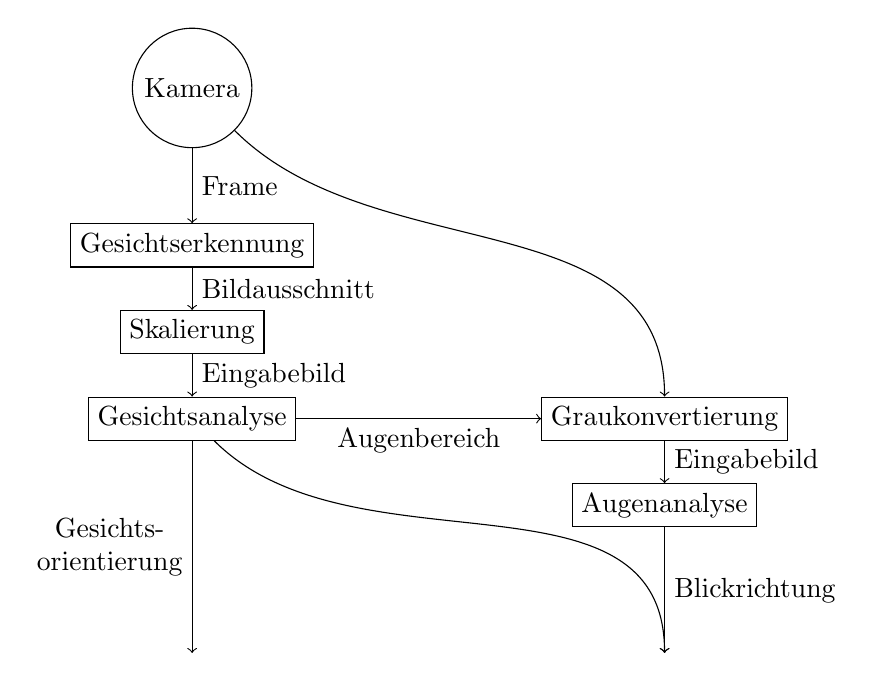
\begin{tikzpicture}
	\node[circle,draw,align=center] (C) at(0,0) {Kamera};
	\node[draw,align=center] (F) at(0,-2)  {Gesichtserkennung};
	\node[draw,align=center] (S) at(0,-3.1)  {Skalierung};
	\node[draw,align=center] (G) at(6,-4.2)  {Graukonvertierung};
	\node[draw,align=center] (A) at(0,-4.2)  {Gesichtsanalyse};
	\node[draw,align=center] (E) at(6,-5.3)  {Augenanalyse};
	
	\node (outA) at(0,-7.3)  {};
	\node (outB) at(6,-7.3)  {};
	
	\draw[->] (E)to node[right,align=center]{Blickrichtung}(outB);
	\draw[->] (A)to[out=-45,in=90] node[right]{}(outB);
	
	\draw[->] (C)to node[right]{Frame}(F);
	\draw[->] (F)to node[right]{Bildausschnitt}(S);
	\draw[->] (S)to node[right]{Eingabebild}(A);
	\draw[->] (A)to node[left,align=center]{Gesichts-\\orientierung}(outA);
	
	\draw[->] (A)to node[below]{Augenbereich}(G);
	\draw[->] (C)to[out=-45,in=90] node[left]{}(G);
	\draw[->] (G)to node[right]{Eingabebild}(E);
\end{tikzpicture}
\end{footnotesize}
\end{center}
\end{frame}
Zur Bestimmung der Blickrichtung sowie Kopfposition und Orientierung wird ein mehrstufiges Verfahren eingesetzt:\\
Zuerst müssen alle Gesichter, die im aktuellen Videobild (Frame) vorhanden sind, detektiert werden, siehe \autoref{MTCNN}. Dabei machen die relevanten Bereiche nur einen sehr geringen Anteil des gesamten Bildes aus.\\
Da Gesichtserkennung und Landmark Erkennung auf unterschiedlichen großen Gesichtsbereichen arbeiten (z.B. Haare und Kinn teilweise als Gesicht zählen, teilweise nicht) ist ein Zwischenschritt zur Vergrößerung der erkannten Bereiche notwendig, damit das gesamte Gesicht abgebildet ist.\\
Ist ein Gesicht in mehreren Einzelnbildern des Videos abgebildet, so muss auch eine Identitätszuordnung vorgenommen werden, damit dem Computerprogramm bekannt ist welches Gesicht in Bild 1 welchem in Bild 2 entspricht. Für die Zuordnung reicht es meist aus, jene Box zu wählen, die am ehesten den selben Bildausschnitt repräsentiert entweder über ähnliche Positionierung im Videobild oder über die Bildähnlichkeit da ein Kopf zwischen zwei schnell aufeinanderfolgenden Einzelbildern nur limitiert bewegen kann.\\
Damit sicher auf allen Gesichtern gerechnet werden kann, ist eine semiautomatische Korrektur erforderlich um Falsch-Detektionen zu entfernen und fehlende Boxen der Gesichter ergänzen zu können. Daher können alle bisher unternommenen Schritte auch von anderen Verfahren übernommen werden, da es sich hierbei nur um ein Vorverarbeitungsschritt handelt und zur Beschleunigung sowie Stabilität der späterer Berechnung beitragen soll.\\
Damit das Verfahren im nächsten Schritt zuverlässig arbeiten kann, werden alle zu kleinen Bildbereiche hochskaliert, um die Gesichter auf eine Mindestgröße zu bringen, siehe \autoref{scale_Algos}\\
Diese Bildbereiche werden nun von OpenFace weiterverarbeitet um die Landmarks, die signifikanten Punkte eines Gesichtes, zu bestimmen. Durch die vorherige Identitätszuordnung der Gesichter kann das Verfahren gezielt auf einzelnen Personen arbeiten und ein entsprechend auf die Person eingestelltes CLNF verwenden, um bessere Ergebnisse zu erzielen, siehe \autoref{OpenFace}. Außerdem können alle gefundenen Personen gleichzeitig (parallel) ausgewertet werden.\\
Für dem im nächsten Schritt verwendeten ElSe Algorithmus muss der Bildausschnitt des Auges in ein Graubild umgewandelt werden, siehe \autoref{Graubild}.\\
Um die Position der Pupille noch exakter zu ermitteln wird ElSe verwendet, da durch eine exakte Bestimmung der Pupillenposition, auch eine genaue Blickrichtungsbestimmung möglich ist, siehe \autoref{ElSe}.\\
Nun wird auf Basis der Landmarks und Kameraparameter die Position und Orientierung der Gesichter sowie die Blickrichtung bestimmt, siehe \autoref{calc_Position}.